\section{}
\[
H(s)=\frac{100}{s^2+s+100}\,.
\]
\subsection{Bode-Diagramm}
\begin{center}
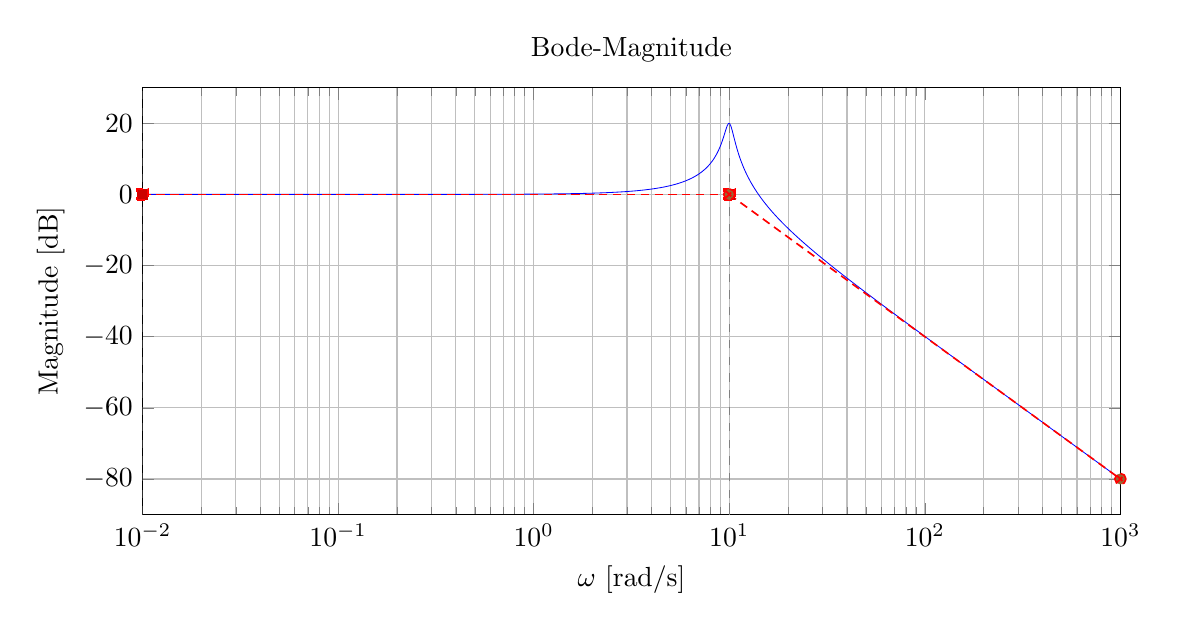
\begin{tikzpicture}
\begin{semilogxaxis}[
  width=14cm,height=7cm,
  xmin=1e-2,xmax=1e3,
  xlabel={$\omega$ [rad/s]},
  ylabel={Magnitude [dB]},
  ytick distance=20,
  grid=both,
  title={Bode-Magnitude}
]
\addplot[
  domain=1e-2:1e3,
  samples=800,
  mark=none,
  line width=0.3pt,
  blue
] {-10*ln((1 - (x/10)^2)^2 + (x/100)^2)/ln(10)};
\addplot+[domain=1e-2:1e1,samples=2,dashed,dash pattern=on 3pt off 2pt,line width=0.6pt,red] {0};
\addplot+[domain=1e1:1e3,samples=2,dashed,dash pattern=on 3pt off 2pt,line width=0.6pt,red] {-40*ln(x/10)/ln(10)};
\draw[gray,dashed] (rel axis cs:0,0) -- (rel axis cs:0,1);
\draw[gray,dashed] (axis cs:10,\pgfkeysvalueof{/pgfplots/ymin}) -- (axis cs:10,\pgfkeysvalueof{/pgfplots/ymax});
\node[gray,anchor=south east] at (axis cs:10,\pgfkeysvalueof{/pgfplots/ymax}) {\scriptsize Polpaar $\omega_n=10$, $\zeta=0.05$};
\end{semilogxaxis}
\end{tikzpicture}
\vspace{6mm}
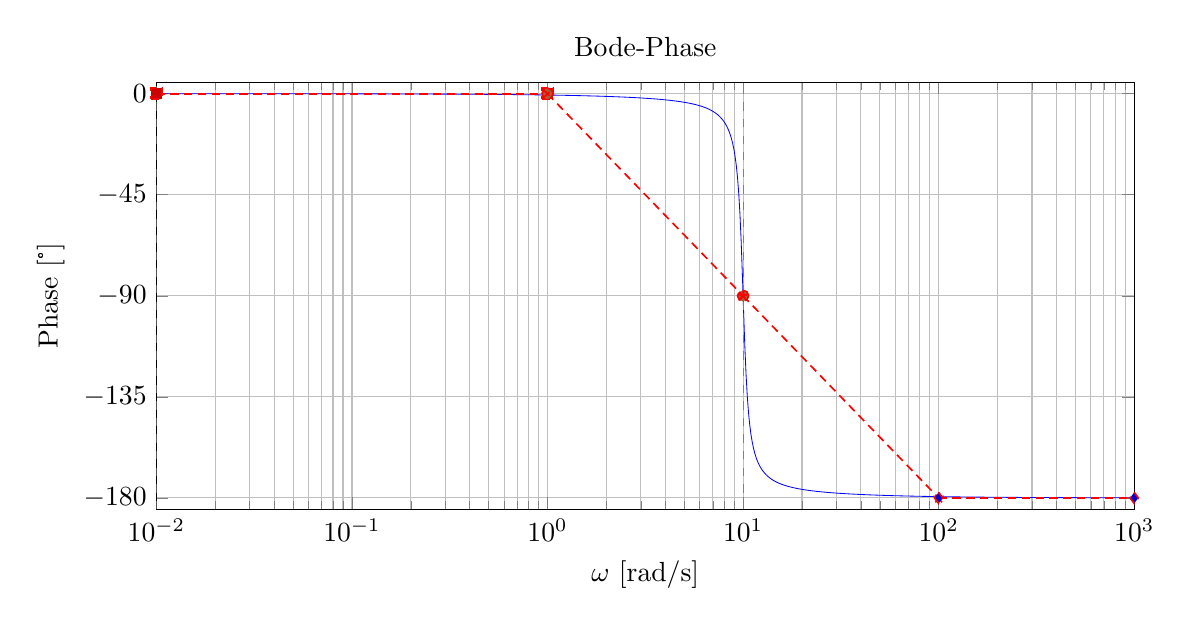
\begin{tikzpicture}
\begin{semilogxaxis}[
  width=14cm,height=7cm,
  xmin=1e-2,xmax=1e3,
  ymin=-185,ymax=5,
  ytick distance=45,
  xlabel={$\omega$ [rad/s]},
  ylabel={Phase [°]},
  grid=both,
  title={Bode-Phase}
]
\addplot[
  domain=1e-2:1e3,
  samples=800,
  mark=none,
  line width=0.3pt,
  blue
] {-atan2(x/100, 1 - (x/10)^2)};
\addplot+[domain=1e-2:1e0,samples=2,dashed,dash pattern=on 3pt off 2pt,line width=0.6pt,red] {0};
\addplot+[domain=1e0:1e1,samples=2,dashed,dash pattern=on 3pt off 2pt,line width=0.6pt,red] {-90*ln(x)/ln(10)};
\addplot+[domain=1e1:1e2,samples=2,dashed,dash pattern=on 3pt off 2pt,line width=0.6pt,red] {-90 - 90*ln(x/10)/ln(10)};
\addplot+[domain=1e2:1e3,samples=2,dashed,dash pattern=on 3pt off 2pt,line width=0.6pt,red] {-180};
\draw[gray,dashed] (rel axis cs:0,0) -- (rel axis cs:0,1);
\draw[gray,dashed] (axis cs:10,\pgfkeysvalueof{/pgfplots/ymin}) -- (axis cs:10,\pgfkeysvalueof{/pgfplots/ymax});
\node[gray,anchor=south east] at (axis cs:10,\pgfkeysvalueof{/pgfplots/ymax}) {\scriptsize Polpaar $\omega_n=10$, $\zeta=0.05$};
\end{semilogxaxis}
\end{tikzpicture}
\end{center}
\newpage
\subsection{Erklärung (ausführlich)}
\begin{description}[leftmargin=1.2em,labelsep=.6em,font=\bfseries]

\item[1. Normalform herstellen.]
Bringe die Übertragungsfunktion exakt in die im Skript definierte Standardform für reelle Pol-/Nullstellen.
\[
H(s)=K_0\cdot s^{\,r}\cdot\frac{1}{1+2d_nT_{p}\cdot s + T_{p}^2\cdot s^2}
\quad.
\]
Hier haben wir: \[
\underline{F}_1(s)=\frac{1}{1+2d_nT_{p}\cdot s + T_{p}^2\cdot s^2},\quad K_0 = \frac{100}{100}=1,\]\[\quad T_p=\frac{1}{10}, \quad d_n=\frac{1}{20}\quad \text{und}\quad r = 0.
\]
\vspace{0.2cm}
Klassifizikation des ersten Teilglieds $\underline{F}_1$: konjugiertes komplexes Polpaar zweiter Ordnung.

\item[2. Eckfrequenz bestimmen und sortieren.]
Bestimme die Eckfrequenz aus der Normform:
\[
\omega_n=\frac{1}{T_p}=10\,\mathrm{rad/s}
\]
Es existiert nur diese charakteristische Frequenz; die aufsteigende Sortierung \(\omega_1<\omega_2<\dots\) ist damit trivial. 

\item[3. Startpunkt des Amplitudengangs festlegen (Geradennäherung).]
Setze die Startfrequenz gleich der kleinsten Eckfrequenz \(\omega_{\min}=\omega_n = 10\,\mathrm{rad/s}\). Verwende die Regel im Skript
\[
F_{\mathrm{dB}}(\omega_{\min})=20\log_{10}\!\Big(|K_0\,F^*_{ges}(0)|\cdot\,\omega_{\min}^{\,r}\Big) = 20 \log_{10}(1) = 0\,\mathrm{dB}.
\]
Dieser Punkt dient als Anker für die Geradennäherung (ohne Resonanzüberhöhung). 

\item[4. Verlauf links vom Startpunkt zeichnen.]
Für \(\omega<\omega_{\min}\) bleibt die Amplituden-Asymptote waagrecht, denn die Anfangssteigung beträgt \(r\cdot 20\,\mathrm{dB/dec}=0\). Trage also eine horizontale Linie bei \(0\,\mathrm{dB}\) ein. 

\item[5. Steigungswechsel an der Eckfrequenz eintragen.]
Ein konjugiertes Polpaar zweiter Ordnung reduziert die Steigung ab \(\omega_n\) um \(40\,\mathrm{dB/dec}\). Da bis jetzt die Steigung \(0\,\mathrm{dB/dec}\) betrug, ist diese ab jetzt \(-40\,\mathrm{dB/dec}\). Zeichne rechts von \(\omega_n\) die Gerade mit Steigung \(-40\,\mathrm{dB/dec}\). Die Formel für die Geradennäherung lautet:
\[
|H(j\omega)|_{\mathrm{dB}}\approx -40\log_{10}\!\Big(\frac{\omega}{\omega_n}\Big)\quad(\omega\ge \omega_n=10).
\]

\item[6. Eckabrundung korrekt berücksichtigen.]
Da $d_n \ll \tfrac{1}{2}$ müssen wir beim Abrunden eine Resonanzüberhöhung mit einbeziehen. Laut Skript erreicht der Magnitudengang bei $\omega = \omega_n$ eine Überhöhung von

\[
-20\log_{10}(2d_n)= -20\log_{10}(\tfrac{1}{10})=20\,\mathrm{dB}
\]
über der asymptotischen \(0\,\mathrm{dB}\)-Gerade. Trage dort einen Stützpunkt und runde die Ecke mit Resonanz entsprechend aus. 

\item[7. Phasenstartwert festlegen.]
Da \(K_0F_{ges}(0)>0\) und \(r=0\), ist der Startwert der Phase
\[
\varphi(0)=r\cdot90^\circ=0^\circ.
\]

\item[8. Phasenänderung durch das Polpaar eintragen.]
Ein komplexes Polpaar zweiter Ordnung erzeugt insgesamt eine Phasenänderung von \(-180^\circ\). Trage die Näherung ein:
\[
\varphi(\omega)\approx
\begin{cases}
0^\circ,& \omega\le 10^{-1}\omega_n\;(=1),\\
\text{linear }-90^\circ/\text{Dec},& 10^{-1}\omega_n<\omega<\omega_n,\\
\text{linear }-90^\circ/\text{Dec},& \omega_n<\omega<10\,\omega_n,\\
-180^\circ,& \omega\ge 10\,\omega_n\;(=100).
\end{cases}
\]
Das lineare Zwischenstück kann formelkonform als \(\varphi(\omega)\approx -90^\circ\log_{10}\omega\) in \([1,10]\) und \(\varphi(\omega)\approx -90^\circ-90^\circ\log_{10}(\omega/10)\) in \([10,100]\) dargestellt werden. 

\item[9. Grenzwerte und Konsistenz prüfen.]
DC: \(|H(0)|=1\Rightarrow 0\,\mathrm{dB}\), \(\varphi(0)=0^\circ\). HF: \(|H(j\omega)|\sim 100/\omega^2\Rightarrow -40\log_{10}(\omega/10)\,\mathrm{dB}\). Pol-/Nullzählung bestätigt die Endphase: Zählergrad \(m=0\), Nennergrad \(n=2\Rightarrow \varphi(\infty)=(m-n)\cdot 90^\circ=-180^\circ\). 

\end{description}

\subsubsection*{Stückweise Näherungen (für die Skizze)}
\[
|H(j\omega)|_{\mathrm{dB}}\approx
\begin{cases}
0,& \omega\ll 10,\\[2pt]
+20,& \omega=10,\\[2pt]
-40\log_{10}(\omega/10),& \omega\gg 10,
\end{cases}
\qquad
\]
\[
\varphi(\omega)\approx
\begin{cases}
0^\circ,& \omega\le 1,\\[2pt]
-90^\circ\log_{10}\omega,& 1<\omega<10,\\[2pt]
-90^\circ-90^\circ\log_{10}(\omega/10),& 10<\omega<100,\\[2pt]
-180^\circ,& \omega\ge 100.
\end{cases}
\]

\newpage